
\chapter{Introduction}


\hspace{1cm}This chapter provides an overview of the study, covering the challenges of the campus library, the study’s objectives, and its significance. It defines the problem, outlines research goals, and highlights the proposed system’s potential impact. The scope and limitations clarify its boundaries, while the project dictionary and notes offer essential terms and supporting details. 

\begin{refsection}
\section{Background of the Problem}
\hspace{1cm}Large Language Models (LLMs) such as OpenAI's ChatGPT \cite{achiam2023gpt}  and Deepseek \cite{guo2025deepseek} have made significant advancements in Natural Language Processing (NLP) by excelling in diverse applications such as conversational chatbots, text summarization \cite{lewis2019bart}, and code summarization and generation \cite{nijkamp2022codegen,chen2021evaluating}
 In addition, these advancements have benefited various fields, including academic research. However, LLM responses can depend heavily on the data on which the model was trained, and they cannot retrieve real-time or external information beyond their pre-trained knowledge. This makes them less effective for tasks that require up-to-date, specific institutional data, such as retrieving current academic resources in university libraries \cite{liu2024information}.

\bigbreak
\hspace{0.4cm}Writing an academic paper requires a deep understanding of the subject and a significant amount of related literature for credible evidence, which can be challenging and time-consuming \cite{khalifa2024using}. It is essential to first visit the university library to search and gather existing related literature significant to the researcher’s study.  However, most libraries today still operate in traditional, non-digital formats where materials are only accessible on-site, making the process of finding and retrieving resources more difficult. Furthermore, some school libraries offer limited access and prohibit users from taking home thesis papers. These challenges significantly delay the progress of future academic research due to limited access to relevant literature in university libraries \cite{prajapat2022comparative}. 


\bigbreak
\hspace{0.4cm}To address retrieval issues, several universities in the Philippines have recognized the importance of adopting digital archiving systems to improve academic access. This becomes more evident in the last previous year before covid-19 pandemic, when researchers were unable to access library resources, prompting libraries to adapt and make resources accessible even remotely. However, digitalization alone does not fully solve the problem \cite{aydin2021comparing, lagas2023challenges, prajapat2022comparative}. Unfortunately, most digitalized libraries today still use outdated search systems that need an exact keyword search, which can result in irrelevant materials \cite{setiyani2023increasing}. The current search mechanism of this digital archives including the Camarines Sur Polytechnic Colleges (CSPC) library still heavily depends on traditional keyword-matching algorithms. If users do not input the exact title or precise keywords, the system returns "not found" even when relevant content exists. This limitation highlights a deeper issue in search functionality, where vague or topic-based queries cannot retrieve appropriate materials, thereby hindering access to valuable research. This inefficiency in retrieval presents a serious barrier for the academe community,  particularly when conducting time-sensitive or exploratory academic work.

\bigbreak
\hspace{0.4cm}These challenges of university libraries in the Philippines, including the CSPC library, have shared difficulties in accessing academic resources, outdated search systems, and ineffective information retrieval that affect the efficiency of academic research. While numerous studies have also explored the integration of the emerging LLM-powered chatbots in academic research \cite{aboelmaged2024conversational}, their implementation and effect for thesis retrieval in specific university libraries, including CSPC, have not been established. This is primarily due to the limitations of LLMs, which rely solely on pre-trained knowledge and are unable to access or utilize the unique local archives maintained by individual libraries \cite{bommasani2021opportunities, strich2024improving}.

\bigbreak
\hspace{0.4cm}To overcome these challenges, Retrieval-Augmented Generation (RAG) has emerged as a superior approach \cite{lewis2020retrieval}. Unlike standalone LLMs, which require retraining and additional domain-specific data to adjust LLM weights, RAG presents an advanced approach by retrieving relevant external information to generate responses and holds significant practical implications for university libraries by improving search functionalities. Additionally, RAG ensures that the most relevant academic resources are retrieved quickly and straightforwardly, making it suitable for libraries with expansive collections of academic papers that are difficult for researchers and students to navigate \cite{wang2024mememo, huang2023retrieval}.

\bigbreak
\hspace{0.4cm}This thesis proposes an enhanced LLM-powered chatbot with the integration of the Retrieval-Augmented Generation (RAG) technique to improve information retrieval, especially in literature search and thesis retrieval of university-owned thesis PDFs at the Camarines Sur Polytechnic Colleges (CSPC) Library. This chatbot application will generate answers and retrieve relevant documents based on the user's prompt.

% \begin{figure}[ht]
%     \centering
% 	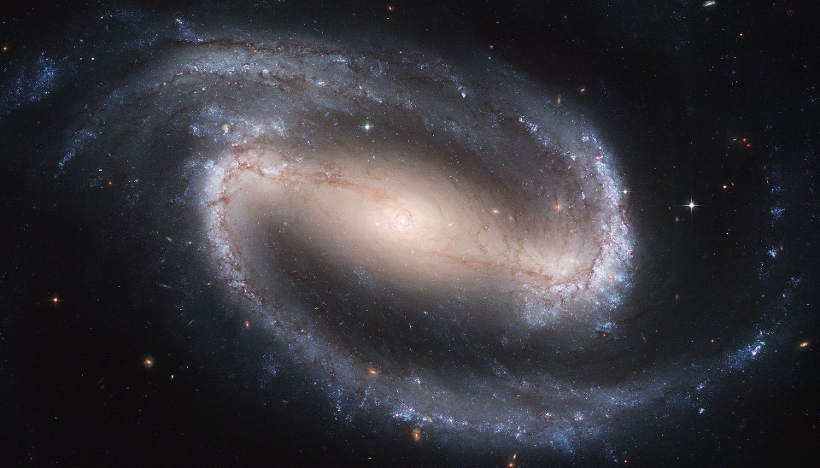
\includegraphics[width=0.85\textwidth]{figures/sampleFig1.jpg} 
% 	\caption[Barred spiral galaxy NGC 1300]{Barred spiral galaxy NGC 1300 photographed by Hubble telescope. While the galaxy in the photo is not our sun, it does emit light, much like our sun. Image credit: NASA.}
% 	\label{fig:firstFig}
% \end{figure}

% The stars in the sky are of particular interest to the aptly named , which in many recent experiments has shown promising results in converting this energy in a non-photoelectric sense into usable energy \cite{ssdsdsd_solid_2012}. Interestingly, \gls{starlabs} has theorized that the famous superhero known as ``Superman'' converts the light from our sun, which grants his fantastic abilities. There are many methods in industry for converting the sun's energy (of about \SI{1000}{\watt\per\meter\squared}) into electrical energy. Some of these are highlighted in \ref{tbl:sampleTbl1} \cite{noauthor_techopedia_nodate}.

% \begin{table}[ht]
% \centering
% \caption{This is a table}
% \label{tbl:sampleTbl1}
% \resizebox{0.8\textwidth}{!}{%
% \begin{tabular}{llll}
% \hline
% installation & type & capacity (GW) & location \\ \hline
% Longyangxia Dam & photovoltaic & 0.85 & China \\
% Gansu Wind Farm & wind & 6 & China \\
% Sihwa Lake & tidal & 0.254 & South Korea \\ \hline
% \end{tabular}%
% }
% \end{table}

\section{Statement of the Problem}

% Enter the statement of the problem here. To cite a study add a bib entry in the references.bib, then use this code \cite{noauthor_biblatex_nodate} to cite the study.

\hspace{1cm}Finding relevant thesis literature in a University's library, such as in CSPC, can be challenging. Many researchers in the academic community struggle to find the exact thesis paper they need, often requiring them to travel and physically visit the library just to retrieve specific documents.

\bigbreak
\hspace{0.4cm}Currently, CSPC’s library website [25] only allows users to search by exact document title. Finding relevant research becomes difficult if users don’t know the exact title. Furthermore, library policies restrict users from taking thesis books outside the premises, limiting accessibility to essential academic resources.  In response to these challenges, this study aims to explore creating a chatbot that eliminates those limitations by enabling searches based on topics, keywords, or even vague descriptions. Additionally, we aim to make this available everywhere. This goal, with the use of the Retrieval Augmented Generation (RAG) algorithm, will revolutionize how the academe community interacts with the CSPC library, making research faster, smarter, and more user-friendly. 

% \begin{enumerate}
%     \item How can the integration of Retrieval-Augmented Generation (RAG) enhance the retrieval of thesis documents from CSPC's digital archives?
%      \item In what ways can a RAG-powered chatbot facilitate natural language queries to deliver context-aware and summarized results, thereby improving research efficiency?
%     \item How can the system support full-text retrieval and provide intelligent filtering options (e.g., by author, year, or topic) to streamline literature discovery for CSPC students and faculty?
% \end{enumerate}
\section{Objectives of the Study}
\hspace{0.4cm}The objectives of this study are divided into two categories: general and specific. The general objective defines the overall goal of the study, while the specific objectives break down this goal into measurable and achievable steps. These objectives ensure a structured approach to developing an enhanced LLM chatbot for Camarines Sur Polytechnic Colleges. 

\subsection{General Objective}
The general objective of this study is to develop a chatbot for  Camarines Sur Polytechnic Colleges (CSPC) library, using Retrieval-Augmented Generation (RAG) to enhance thesis retrieval and literature search in CSPC Library, replacing the traditional keyword-based search with a more conversational and topic-oriented search and response approach.

\subsection{Specific Objectives}
To achieve the general objective, the study sets the following specific objectives:
\begin{enumerate}
    \item To integrate a document ingestion and retrieval module for storing thesis documents.
    \item To Implement a semantic search and thesis document retrieval system using RAG and Deepseek R1 LLM.
    \item To Evaluate the performance of the RAG chatbot using RAGASS.
    \item To Deploy the RAG chatbot on a local server
\end{enumerate}

% \begin{enumerate}
%     \item To write this research paper
%     \item To present it in the title defense.
% \end{enumerate}
   
\clearpage
\section{Significance of the Study}

The result of this study will benefit the following:

\bigbreak
\noindent \textbf{Students.}  By integrating semantic search and retrieval capabilities, the chatbot will significantly improve search accuracy and efficiency, reducing the time spent on literature review. This will enable students and researchers to quickly find relevant studies without relying solely on exact keywords or titles.

\bigbreak
\noindent \textbf{Faculty Members.}  The chatbot will serve as a research aid for faculty members by providing easier access to relevant studies. This will enhance their ability to aid students in thesis writing, academic guidance, and collaborative research work, while at the same time reducing the extent of manual effort in literature searching.

\bigbreak
\noindent \textbf{CSPC Library Management.} The implementation of a RAG-powered chatbot will modernize the library’s digital infrastructure, making academic resources more accessible to users. By automating thesis retrieval and search functions, the system will improve library service and optimize resource utilization.

\bigbreak
\noindent \textbf{Researchers.} The study will contribute to the field of AI-driven academic search and retrieval, providing insights into the practical applications of Retrieval-Augmented Generation (RAG). Future researchers can build on this work by exploring ways to further optimize search relevance, retrieval efficiency, and integration with other AI models.

\section{Scope and Limitation}

\hspace{1cm}The scope of this study is to develop a chatbot for the Camarines Sur Polytechnic Colleges (CSPC) library, utilizing Retrieval-Augmented Generation (RAG) with the Deepseek R1 LLM. The goal is to address the challenges faced by the academic community in searching and retrieving thesis literature by replacing the current yet traditional keyword-based search with a more conversational and topic-oriented approach. This will be done through a website based with an access control where admin can upload new published pdf thesis and users can register through their cspc email. Additionally, we aim to deploy this on a local server. This project will be conducted over two whole semesters, allowing ample time for development and testing.

\bigbreak
\hspace{0.4cm}There are certain limitations to consider in this study. First, our team will focus only on utilizing the available PDF copies of undergraduate theses that have already been published. Second, the chatbot’s accuracy will depend on the quality and structure of thesis records, and on the clarity and relevance of the user's prompts. Additionally, hardware limitations may constrain computational efficiency, which could affect the chatbot’s real-time processing capabilities. Finally, while the RAG technique can reduce hallucination, users are advised to validate the outputs carefully as occasional inaccuracies or fabricated information may still occur. 


\section{Project Dictionary}

The Project Dictionary contains the technical terms that defined the conceptual and operation of this study:

\begin{itemize}
    \item \textbf{Academic Literature Retrieval.} The process of systematically searching for and obtaining scholarly documents, such as research papers and theses, to support academic work \cite{sallam2023chatgpt}. In this study, the implementation of LLMs is essential to improve the retrieval of academic literature.
    \item \textbf{Chatbot.} An AI-powered conversational agent designed to interact with users in natural language, providing assistance, answering queries, and facilitating access to information in a user-friendly manner \cite{chow2023developing}. In this study, chatbots will be implemented for answering questions with human-like responses.
    \item \textbf{CSPC Library.} The Camarines Sur Polytechnic Colleges (CSPC) Library serves as the primary academic resource center for students and faculty. It offers access to a diverse collection of books and theses inside the premises. The library has initiated steps toward digitalization, providing an online catalog for users to search materials. In this study, the CSPC Library is examined to assess its current digital infrastructure and explore enhancements to improve information retrieval and user experience.
    \item \textbf{Generative AI.} A kind of artificial intelligence that may produce original text, graphics, or code, frequently in response to a user-inputted prompt. More and more online applications and chatbots that let users enter instructions or inquiries into an input box are using its models. The AI model will produce a response in the output field that resembles a human response \cite{bozkurt2024genai}. In this study, we will examine the implications of Generative AI in the education and academic integrity context.
    \item \textbf{Large Language Models (LLMs).} AI models trained on vast text datasets to understand and generate human-like responses. They excel in natural language tasks but struggle with retrieving real-time and domain-specific information \cite{klang2024advancing}. In this study, the implementation of the Large Language Model (LLM) streamlines access to information, assists in literature searches, and facilitates query handling effectively.
    \item \textbf{Natural Language Processing (NLP).} A subfield of artificial intelligence (AI) called natural language processing (NLP) makes it possible for computers to comprehend and understand spoken, written, or even handwritten human language. NLP is essential to enabling seamless and organic human-computer interactions as AI-driven technologies grow more pervasive in daily life \cite{ramirez2024natural}. In this study, NLP significantly improves machine comprehension to understand human language and improves user interaction through chatbots.
    \item \textbf{Retrieval-Augmented Generation (RAG).} An AI framework that enhances LLMs by incorporating an external knowledge retrieval mechanism, improving the accuracy and contextual relevance of generated responses \cite{lewis2020retrieval}. In this study, RAG will be developed for navigating and retrieving information from large amounts of academic papers.
    \item \textbf{Semantic Search.} A search approach that goes beyond keyword matching by understanding the intent and contextual meaning of queries to return more relevant results \cite{mahboub2024evaluation}. In this study, semantic search will significantly improve the performance of RAG in generating relevant and contextual responses due to the enhanced retrieval process by understanding user queries which is beneficial for the CSPC library that holds a large collection of academic papers.
\end{itemize}

%=======================================================%
%%%%% Do not delete this part %%%%%%
\clearpage

\printbibliography[heading=subbibintoc, title={\centering Notes}]
\end{refsection}